
\begin{figure}[t]
\centering

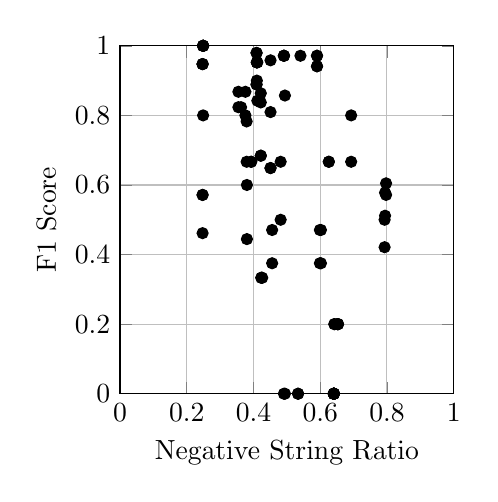
\begin{tikzpicture}
\begin{axis}[
    width=0.48\linewidth,
    height=6cm,
    xlabel={Negative String Ratio},
    ylabel={F1 Score},
    xmin=0, xmax=1,
    ymin=0, ymax=1,
    grid=both,
]
\addplot[
    only marks,
    mark=*,
]
coordinates {
(0.3759,0.8000) (0.3759,0.8679) (0.3549,0.8235) (0.3549,0.8679) (0.3629,0.8235) (0.4102,0.9524) (0.4102,0.9524) (0.4102,0.9524) (0.4102,0.9000) (0.4117,0.9524) (0.4117,0.8421) (0.3932,0.6667) (0.3932,0.6667) (0.3804,0.6000) (0.3804,0.4444) (0.3796,0.7826) (0.3796,0.6667) (0.5337,0.0000) (0.5337,0.0000) (0.5905,0.9714) (0.5905,0.9412) (0.4913,0.0000) (0.4913,0.9714) (0.5905,0.9412) (0.4913,0.9714) (0.5905,0.9714) (0.4913,0.9714) (0.5408,0.9714) (0.2492,1.0000) (0.2492,0.8000) (0.2491,1.0000) (0.2491,1.0000) (0.2492,1.0000) (0.2492,1.0000) (0.6408,0.0000) (0.6408,0.0000) (0.6408,0.0000) (0.6408,0.0000) (0.6408,0.0000) (0.6408,0.0000) (0.6408,0.0000) (0.6408,0.0000) (0.6408,0.0000) (0.6408,0.0000) (0.4220,0.6842) (0.4220,0.8372) (0.4512,0.6486) (0.4512,0.8095) (0.4093,0.8889) (0.4093,0.9796) (0.4220,0.6842) (0.4512,0.6486) (0.4093,0.8889) (0.4220,0.8636) (0.4512,0.9583) (0.4093,0.9796) (0.6524,0.2000) (0.6524,0.2000) (0.6425,0.2000) (0.6425,0.2000) (0.6534,0.2000) (0.6534,0.2000) (0.7974,0.5714) (0.7974,0.6047) (0.7944,0.5778) (0.7944,0.5116) (0.7930,0.4211) (0.7930,0.5000) (0.6022,0.3750) (0.6022,0.4706) (0.5991,0.3750) (0.5991,0.4706) (0.4560,0.3750) (0.4560,0.4706) (0.6258,0.6667) (0.6258,0.6667) (0.6928,0.6667) (0.6928,0.8000) (0.4815,0.5000) (0.4815,0.6667) (0.4237,0.3333) (0.4237,0.3333) (0.4263,0.3333) (0.2476,0.5714) (0.2476,0.9474) (0.2476,0.5714) (0.2476,0.9474) (0.2476,0.4615) (0.2476,0.9474) (0.4943,0.0000) (0.4943,0.8571)
};
\end{axis}
\end{tikzpicture}
\hfill
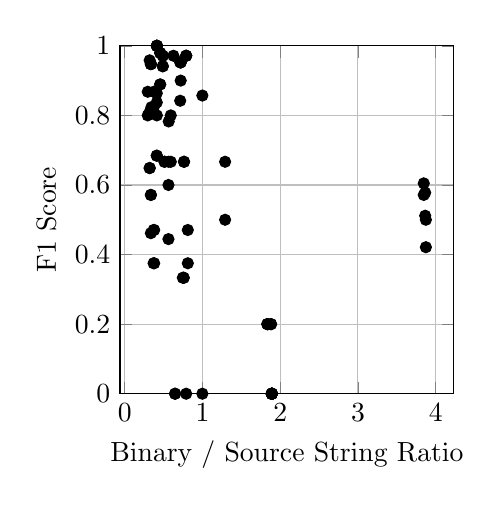
\begin{tikzpicture}
\begin{axis}[
    width=0.48\linewidth,
    height=6cm,
    xlabel={Binary / Source String Ratio},
    ylabel={F1 Score},
    ymin=0, ymax=1,
    grid=both,
]
\addplot[
    only marks,
    mark=*,
]
coordinates {
(0.2968,0.8000) (0.2968,0.8679) (0.3736,0.8235) (0.3736,0.8679) (0.3435,0.8235) (0.7203,0.9524) (0.7203,0.9524) (0.7203,0.9524) (0.7203,0.9000) (0.7141,0.9524) (0.7141,0.8421) (0.5123,0.6667) (0.5123,0.6667) (0.5631,0.6000) (0.5631,0.4444) (0.5661,0.7826) (0.5661,0.6667) (0.6484,0.0000) (0.6484,0.0000) (0.4899,0.9714) (0.4899,0.9412) (0.7908,0.0000) (0.7908,0.9714) (0.4899,0.9412) (0.7908,0.9714) (0.4899,0.9714) (0.7908,0.9714) (0.6268,0.9714) (0.4139,1.0000) (0.4139,0.8000) (0.4143,1.0000) (0.4143,1.0000) (0.4139,1.0000) (0.4139,1.0000) (1.8920,0.0000) (1.8920,0.0000) (1.8920,0.0000) (1.8920,0.0000) (1.8920,0.0000) (1.8920,0.0000) (1.8920,0.0000) (1.8920,0.0000) (1.8920,0.0000) (1.8920,0.0000) (0.4127,0.6842) (0.4127,0.8372) (0.3212,0.6486) (0.3212,0.8095) (0.4566,0.8889) (0.4566,0.9796) (0.4127,0.6842) (0.3212,0.6486) (0.4566,0.8889) (0.4127,0.8636) (0.3212,0.9583) (0.4566,0.9796) (1.8391,0.2000) (1.8391,0.2000) (1.8826,0.2000) (1.8826,0.2000) (1.8348,0.2000) (1.8348,0.2000) (3.8468,0.5714) (3.8468,0.6047) (3.8649,0.5778) (3.8649,0.5116) (3.8739,0.4211) (3.8739,0.5000) (0.3720,0.3750) (0.3720,0.4706) (0.3792,0.3750) (0.3792,0.4706) (0.8119,0.3750) (0.8119,0.4706) (0.7634,0.6667) (0.7634,0.6667) (0.5928,0.6667) (0.5928,0.8000) (1.2917,0.5000) (1.2917,0.6667) (0.7587,0.3333) (0.7587,0.3333) (0.7478,0.3333) (0.3371,0.5714) (0.3371,0.9474) (0.3371,0.5714) (0.3371,0.9474) (0.3369,0.4615) (0.3369,0.9474) (0.9991,0.0000) (0.9991,0.8571)
};
\end{axis}
\end{tikzpicture}

\caption{Impact of string characteristics on macro recovery performance.}
\end{figure}
